\documentclass[9pt]{beamer}
\usepackage[utf8]{inputenc}
\usepackage{pslatex}
%% \usetheme[nat, greybg]{Frederiksberg}
\usetheme[nat]{Frederiksberg}
%% \usetheme[nat,wmark,logoplace=left,style=simple]{Frederiksberg}
%% \usetheme[nat,logoplace=left,style=simple]{Frederiksberg}

\usepackage{amsmath}
\usepackage{amsfonts}
\usepackage{amsthm}
\usepackage{amssymb}
\usepackage{mathtools}


\usepackage{listings}
\usepackage{subcaption}
\usepackage{caption}
\usepackage{subcaption}
\usepackage{verbatim}
\usepackage{multirow}

\DeclarePairedDelimiter\floor{\lfloor}{\rfloor}
\graphicspath{ {imgs/} } 


\title{Breaks For Additive Season and Trend (BFAST)}
\subtitle{Theoretical background and results}
\institute{Department of Computer Science}
\author{Dmitry Serykh}
\date{\today}

\begin{document}

\frame[plain]{\titlepage}

\begin{frame}
\frametitle{The Context}
\begin{itemize}
\item 7.5 ECTS project from Block 5
\item Two variants of the BFAST algorithm:
  \begin{itemize}
  \item The original BFAST (not to be confused with BFAST Monitor)
  \item BFAST0n: a lightweight version of BFAST
  \end{itemize}
\item Describe the underlying theory behind the main algorithm steps
\item Implement BFAST and BFAST0n in Python
\item Validate the implementation on multiple datasets, including datasets from
  the original paper by Verbesselt et al.
\item Foundation for a parallel BFAST implementation in the future
\end{itemize}
\end{frame}

\begin{frame}
  \frametitle{Introduction}
  
\end{frame}

\begin{frame}
  \frametitle{Ordinary Least Squares (OLS) Regression - Quick Recap}
  \begin{itemize}
    \item A crucial component of the BFAST and BFAST0n algorithms
    \item Linear Model
      \[
      \mathrm{Y} = \mathrm{X}\beta + \varepsilon
      \]
    \item Wish to find a solution to a quadratic minimization problem
      \[
      \hat{\beta} = \operatorname{argmin}_{\beta} \|Y-\mathrm{X} \boldsymbol{\beta}\|^{2}
      \]
    \item $\hat{\beta}$ is the OLS estimator for $\beta$ and can be found using the explicit formula:
      \[
      \hat{\boldsymbol{\beta}}=\left(\mathrm{X}^{\top} \mathrm{X}\right)^{-1}\mathrm{X}^{\top} \mathrm{Y}
      \]
    \item A numerically stable solution can be obtained using QR-decomposition or Moore-Penrose
      pseudoinverse of $\mathrm{X}$ (an expansive topic in itself).
  \end{itemize}
\end{frame}

\begin{frame}
\frametitle{OLS-Regression for Non-linear Functions}
\begin{itemize}
\item Linear regression can be used to estimate linear parameters for
  non-linear functions.
\item E.g. $f(x) = 25 + 2x^{1.2} + 3 \sin{x}$, then:
  \[
  \mathrm{X} = 
  \begin{bmatrix}
    1 & x_1^{1.2} & \sin{x_1}\\
    1 & x_2^{1.2} & \sin{x_2}\\
    \vdots & \vdots & \vdots \\
    1 & x_n^{1.2} & \sin{x_n}
  \end{bmatrix}
  \quad
  \beta =
  \begin{bmatrix}
    25 \\
    2 \\
    3
  \end{bmatrix}
  \]
\end{itemize}
\end{frame}


\begin{frame}
  \frametitle{OLS Example}
  \begin{figure}[H]
    \centering
    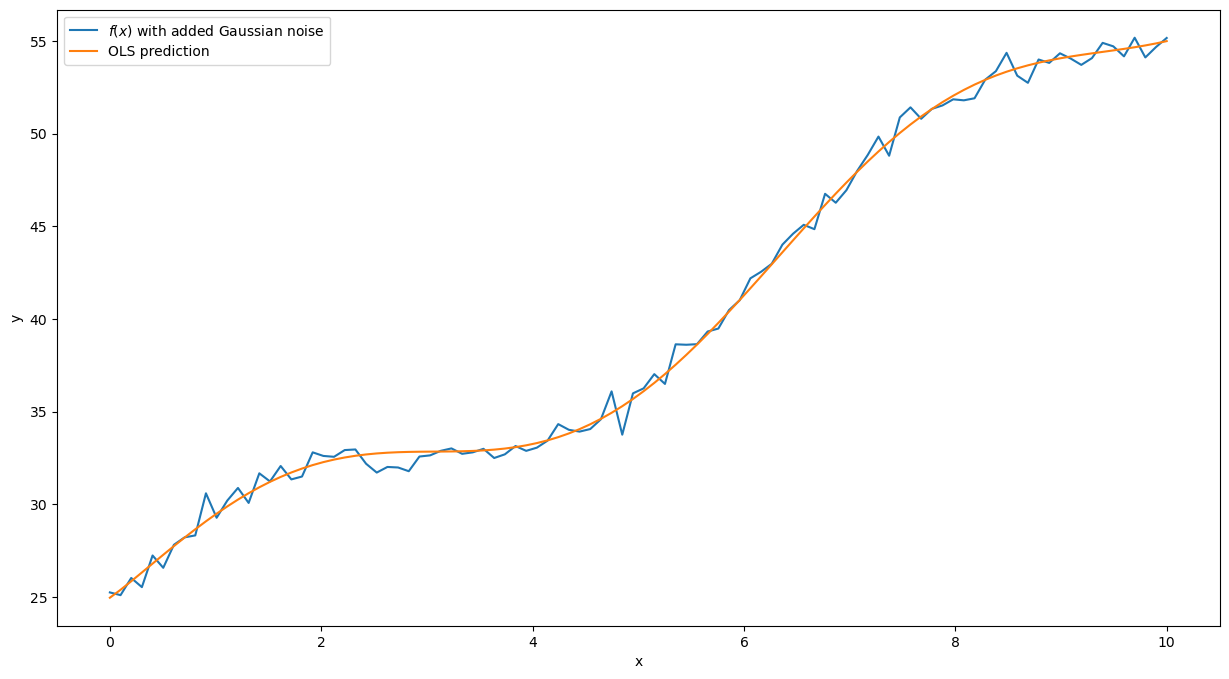
\includegraphics[width=0.8\textwidth]{imgs/ols1.png}
  \end{figure}
\end{frame}

\begin{frame}
\frametitle{STL Intro}
\begin{itemize}
\item Seasonal and Trend decomposition using Loess (STL), as first described by Cleveland et al.
\item Decomposition of a time series ($Y_v$) into a trend ($T_v$), seasonal ($S_v$) and remainder
  ($R_v$) s.t:
  \[
  Y_v = T_v + S_v + R_v \text{ for } v \in 1 \hdots N
  \]
\end{itemize}
\end{frame}

\begin{frame}
  \frametitle{STL Example}
  \begin{figure}[H]
    \centering
    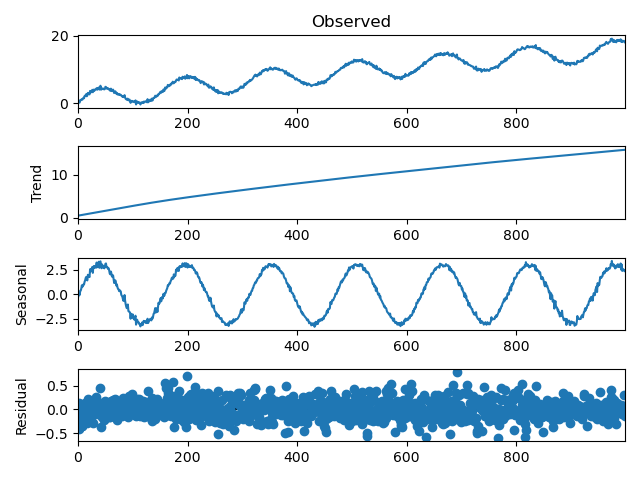
\includegraphics[width=0.7\textwidth]{imgs/stl1.png}
    \caption{$f(x) = x^{0.75} + 2\sin(x)$ with added noise
      $\sim \mathcal{N}(0, 0.25)$}
  \end{figure}
  \centering
\end{frame}


\begin{frame}
\frametitle{Locally Estimated Scatterplot Smoothing (LOESS)}
\begin{itemize}
  \item For all $x$ fit a curve $\hat{g}(x)$ by giving the other points $x_i$ a
  weight $v_i$.
\item Select the value of the smoothing factor $q \in \mathbb{Z}^+$ and let
  $\lambda_q(x)$ be the distance from $x$ to q'th closest $x_i$. For $q > n$:
  \[
  \lambda_q(x) = \frac{q \cdot \lambda_n(x)}{n}
  \]
\item We calculate the weights using the tricube weight function:
  \[
  v_i = \left( 1 - \left( \frac{| x_i - x |}{\lambda_q(x)}  \right)^3\right)^3
  \]
  for $| x_i - x | \geq \lambda_q(x)$, set $v_i = 0$
\item Use locally-linear or locally quadratic fitting with weights
  $\rho_i v_i$, where $\rho_i$ are the robustness weights that make it possible to 
  ignore the outliers in the dataset.
\item The value of $x$ after the application of LOESS is $\hat{g}(x)$,
\end{itemize}
\end{frame}

\begin{frame}
  \frametitle{LOESS Examples}
  \begin{figure}
    \centering
    \begin{subfigure}[b]{0.49\textwidth}
      \centering
      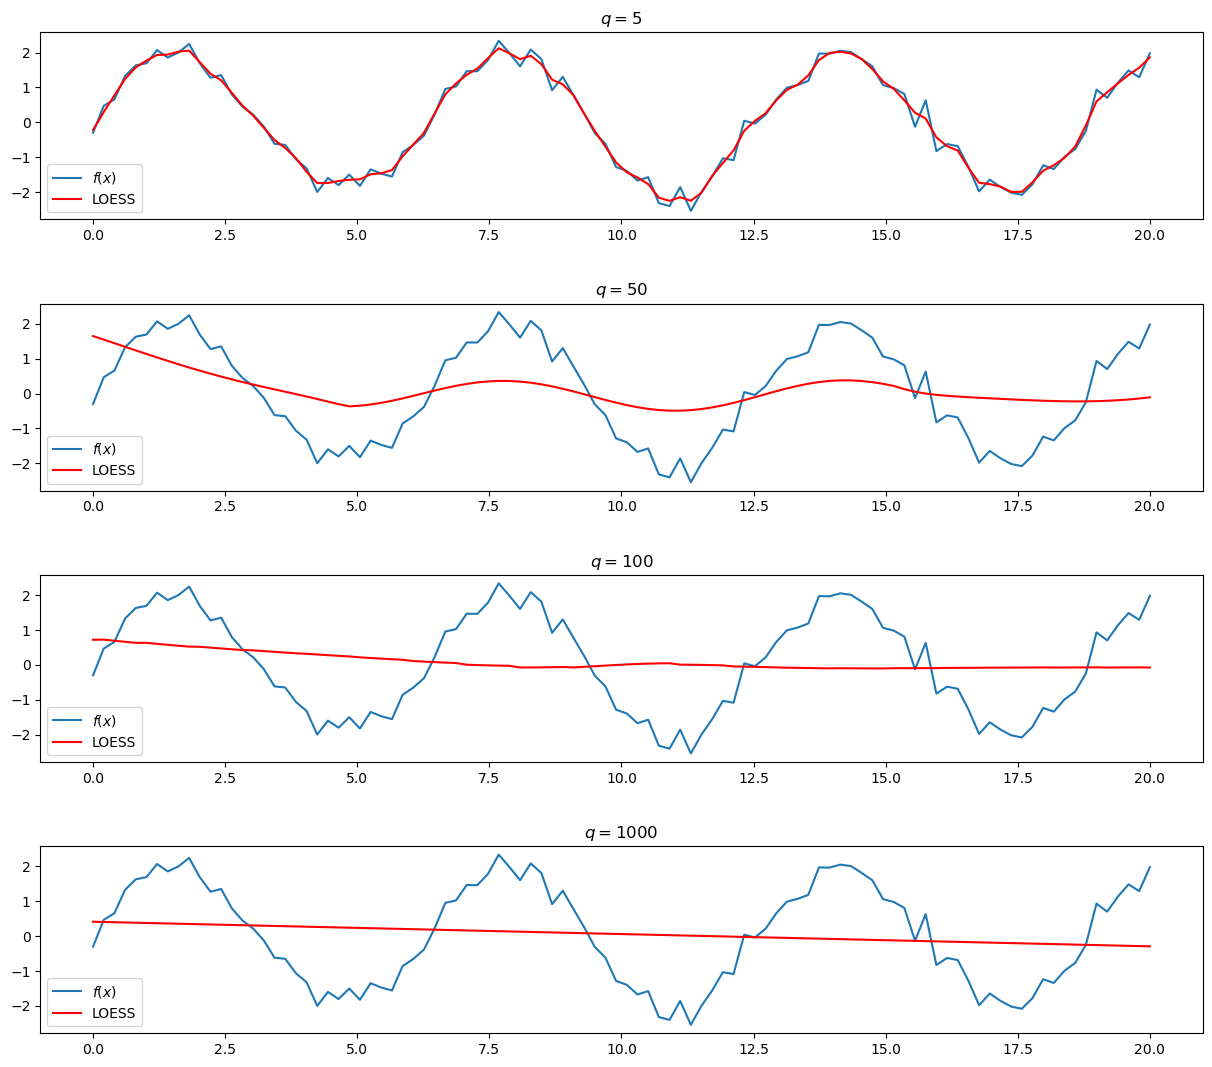
\includegraphics[width=\textwidth]{imgs/loess1}
      \caption{$d=1$}
  \end{subfigure}
  \begin{subfigure}[b]{0.49\textwidth}
    \centering
    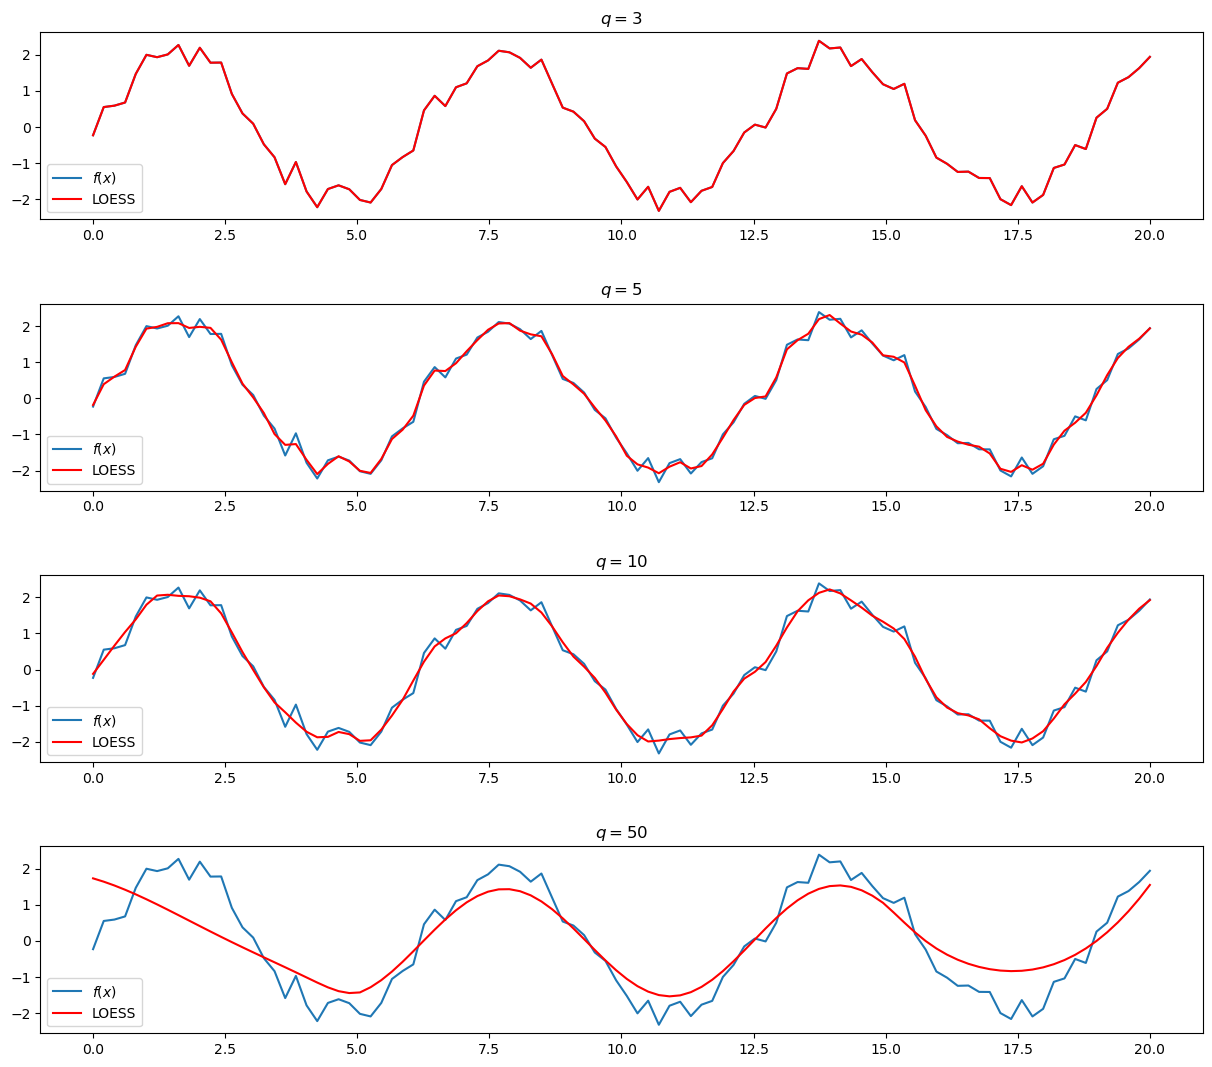
\includegraphics[width=\textwidth]{imgs/loess2}
    \caption{$d=2$}
  \end{subfigure}
  \caption{LOESS applied to $f(x) = 2\sin(x)$ with added Gaussian noise and $n =
    100$. $d$ is the degree of the fitted polynomial}
\end{figure}

\end{frame}

\begin{frame}
  \frametitle{STL Algorithm Steps}
  \begin{itemize}
  \item STL is performed through two nested loops and we begin by setting:
    \[ T_v^{0} = 0, \quad R_v^{0} = 0,  \quad \rho_v = 1 \]
\begin{enumerate}
\item \textbf{Detrending}:
  $V_v = Y_v - T_v^k$, where $k$ is the iteration number of the inner loop
\item \textbf{Cycle-Subseries Smoothing}:
  $V_v$ is split into cycle-subseries, calculate the mean average subseries
  resulting in $C^{k+1}$.
\item \textbf{Low-pass Filter of Smoothed Cycle-Subseries}:
  Apply the low-pass filter to $C_{k+1}$. This is accomplished by application of two
  moving averages of lag equal to 3 followed by LOESS smoothing with $q=n_l$
  and $d=1$. The result is saved as $L^{k+1}$
\item \textbf{Detrending of the Smoothed Cycle-Subseries}:
  $S^{k+1} = C^{k+1} - L^{k+1}$
\item \textbf{Deseasoning}:
  $W_v = Y_v - S_v^k$. 
\item \textbf{Trend Smoothing}:
  Apply LOESS to $W_v$ with $q = n_t$, resulting in $T^{k+1}$
\end{enumerate}
  \end{itemize}
\end{frame}

\begin{frame}
  \frametitle{STL Algorithm Steps - Continued}
  \begin{itemize}
\item  The outer loop consists of following steps:
  \begin{enumerate}
  \item Run the inner loop
  \item Find the remainder, ($T_v$ and $S_v$ are from the last iteration of the inner loop):
    $R_v = Y_v - T_v - S_v$
  \item Calculate the robustness weights from the remainder component:
    \[
    \rho_{v}= B\left( \frac{|R_v|}{6\cdot\text{median}(|R_v|)} \right)
    \]
    where $B$ is the bisquare weight function:
    \[
    B(x) =
    \begin{cases}
      \left(1-x^{2}\right)^{2} & \text{ for } 0 \leqslant x<1 \\
      0                     & \text{ for } x>1
    \end{cases}
    \]
\end{enumerate}
\item The inner loop is normally ran $2$ times, while the outer loop is ran
  once, unless there are outliers present in the dataset.
\item Return $T_v$, $S_v$ and $R_v$
  \end{itemize}
\end{frame}


\begin{frame}
\frametitle{OLS-MOSUM Test - The Model}
\begin{itemize}
  \item One step of the BFAST algorithm is to detect structural change in the
    trend and seasonal components before we commit to the heavy-weight
    estimation of the number and location of the breakpoints.
  \item For each observation $i \in (1, \ldots, n)$ we consider a following linear model:
    \[
    y_{i}=x_{i}^{\top} \beta_{i}+u_{i}
    \]
    where:
    \begin{itemize}
    \item $x_i = (1,x_{i2}, x_{i3}, ..., x_{ik})^T \in \mathbb{R}^k$
    \item $u_i \in \mathbb{R}$ is the residual term that is independently and identically
      distributed with mean $\mu = 0$ and variance $\sigma^2$.
    \end{itemize}
  \item 
    We can then test for structural change by testing the null hypothesis:
    \[
    H_0:\quad \beta_i = \beta_0 \quad(i=1, \ldots, n)
    \]
\end{itemize}
\end{frame}

\begin{frame}
  \frametitle{OLS-MOSUM Test - Continued}
  \begin{itemize}
  \item $\hat{\beta}^{(n)}$ is the ordinary least squares (OLS) estimate of the
    regression coefficients based on all the observations up to $n$,
  \item 
    Let the OLS residuals (estimates of $u_i$) be defined as:
    \begin{equation} \label{eq:residuals}
      \hat{u}_i = y_i - x_i^T\hat{\beta}^{(n)}
    \end{equation}
    the variance estimate would then be:
    \begin{equation} \label{eq:sigma}
      \hat{\sigma}^{2}=\frac{1}{n-k} \sum_{i=1}^{n} \hat{u}_{i}^{2}
    \end{equation}
  \end{itemize} 
\end{frame}

\begin{frame}
  \frametitle{Empirical Fluctuation Process (OLS-MOSUM)}
  \begin{itemize}
  \item It is possible to detect structural change by analyzing moving sum of residuals ($\hat{u}$)
  \item 
    The resulting empirical fluctuation process consists of a
    sum of a fixed number of residuals in a data interval, which size is determined
    by the value of the parameter $h \in (0,1)$ (bandwidth).
  \item 
  The OLS-based MOSUM process at time $t$ is given by:
  \begin{equation}\label{eq:mosum_og}
    M(t)=\frac{1}{\hat{\sigma} \sqrt{n}}
    \left(\sum_{i=\floor{N_{n} t}+1}^{\left\lfloor N_{n} t\right\rfloor+\lfloor
      n h\rfloor} \hat{u}_{i}\right) \quad(0 \leq t \leq 1-h)
  \end{equation}
  where $N_{n}=(n-\floor{n h}) /(1-h)$ and $\floor{n h}$ is the size of the
  window. 
  \end{itemize}
\end{frame}

\begin{frame}
  \frametitle{Significance Testing}
  \begin{itemize}
  \item 
    A key observation is that if a structural change takes place at $t_0$, the
    OLS-MOSUM path would also have a strong shift at $t_0$.
    We reject the null hypothesis of there being no structural change, when the fluctuation of
    the OLS-MOSUM process becomes too large.
  \item
    In practice, we determine whether the null
    hypothesis can be rejected using a significance test (also called statistical
    hypothesis testing).
  \item 
    First, we calculate the test statistic. For the residual-based OLS-MOSUM
    process, it is defined as:
    \begin{equation} \label{eq:test_statistic_og}
      S_{\text{MOSUM}} = \max(|M(t)|) \quad \text{ for } 0 \leq t \leq (1-h)
    \end{equation}
  \end{itemize}
\end{frame}

\begin{frame}
  \frametitle{Significance Testing - Continued}
  \begin{itemize}
  \item This formulation is not usable in a context of an implementation, since we are working
    with infinite set of real numbers from $0$ to $1-h$.
  \item Another key observation is that $M(t)$ returns $n - \floor{nh} + 1$ unique values for $0 \leq t \leq (1-h)$:
  \item Let:
    \begin{equation} \label{eq:mosum}
      \bar{M}(t') =
      \frac{1}{\hat{\sigma} \sqrt{n}}
      \left(\sum_{i=t}^{t' + \floor{nh}} \hat{u}_i\right)
      \quad(t' = 1,2, \hdots, n - \floor{nh} + 1))
    \end{equation}
  \item Then: 
    $\max(|M(t)|) = \max(|\bar{M}(t')|)$ and we have:
    \begin{equation} \label{eq:test_statistic}
      S_{\text{MOSUM}} = \max(|\bar{M}(t')|) \quad \text{ for } t' \text{ in } 1,2,..,(n - \floor{nh} + 1)
    \end{equation}
  \end{itemize}
\end{frame}

\begin{frame}
  \frametitle{Significance Testing - Continued 2}
  \begin{itemize}
  \item We use the value of $S_{\text{MOSUM}}$ to calculate the probability of getting such
    sample, given that the null hypothesis holds, using the critical values approach.
    The p-value is calculated from the table of
    simulated asymptotic critical values of the Moving Estimate (ME) tests with
    the maximum norm, given by Chu et al. (1995).
  \item  We then compare the resulting
    probability with a chosen confidence interval, which is a value $0 < \alpha < 1$
    \item If the resulting probability is below the
      value of $\alpha$, we reject the null hypothesis, hence a 
      structural change is detected in the time series. 
  \end{itemize}
\end{frame}

\begin{frame}[fragile]
  \frametitle{Table of Critical Values}
  \begin{table}[]
    \centering
\begin{tabular}{|l|l|l|l|l|l|}
\hline
\multirow{2}{*}{$k$}      & \multicolumn{1}{c|}{\multirow{2}{*}{h}} & \multicolumn{4}{c|}{Tail probability}                                                                     \\ \cline{3-6} 
                          & \multicolumn{1}{c|}{}                   & 0.10                     & 0.05                     & 0.025                    & 0.01                     \\ \hline
\multirow{4}{*}{1}        & 0.05                                    & 0.7552                   & 0.8017                   & 0.8444                   & 0.8977                   \\ \cline{2-6} 
                          & 0.10                                    & 0.9809                   & 1.0483                   & 1.1119                   & 1.1888                   \\ \cline{2-6} 
                          & \multicolumn{1}{c|}{...}                & \multicolumn{1}{c|}{...} & \multicolumn{1}{c|}{...} & \multicolumn{1}{c|}{...} & \multicolumn{1}{c|}{...} \\ \cline{2-6} 
                          & 0.50                                    & 1.3560                   & 1.4938                   & 1.6166                   & 1.7663                   \\ \hline
\multirow{4}{*}{2}        & 0.05                                    & 0.7997                   & 0.8431                   & 0.8838                   & 0.9351                   \\ \cline{2-6} 
                          & 0.10                                    & 1.0448                   & 1.1067                   & 1.1634                   & 1.2388                   \\ \cline{2-6} 
                          & \multicolumn{1}{c|}{...}                & \multicolumn{1}{c|}{...} & \multicolumn{1}{c|}{...} & \multicolumn{1}{c|}{...} & \multicolumn{1}{c|}{...} \\ \cline{2-6} 
                          & 0.50                                    & 1.4884                   & 1.6125                   & 1.7266                   & 1.8639                   \\ \hline
\multicolumn{1}{|c|}{...} & \multicolumn{1}{c|}{...}                & \multicolumn{1}{c|}{...} & \multicolumn{1}{c|}{...} & \multicolumn{1}{c|}{...} & \multicolumn{1}{c|}{...} \\ \hline
\end{tabular}
\caption{An excerpt from the table of simulated asymptotic critical values of the
  ME tests with the maximum norm}
\label{table:critvals}
\end{table}
\end{frame}


\begin{frame}[fragile]
  \frametitle{OLS-MOSUM Test - Steps of the Algorithm}
  \begin{enumerate}
  \item \textbf{Calculate $\hat{\beta}^{(n)}$ using OLS-based linear
    regression from matrix $\mathrm{X}$ and vector $y$}
  \item \textbf{Calculate the vector of OLS residuals $\hat{\mu}$}
  \item \textbf{Calculate the standard deviation $\hat{\sigma}$}
  \item \textbf{Calculate the residual-based OLS-MOSUM process as a vector of size $n - \floor{nh} + 1$}
  \begin{verbatim}
  nh = floor(n * h)
  e = concat([0], residuals)
  process = cumsum(e)
  process = process[nh:n] - process[0:(n - nh + 1)]
  process = process / (sigma * sqrt(n))
  \end{verbatim}
\item \textbf{Calculate the test statistic $S_{\text{test}}$} = \texttt{max(abs(process))}
\item \textbf{Calculate the p-value using the table of critical values and linear interpolation}
\item \textbf{Return the result}: \\
  If $p \leq \alpha$, we reject the null-hypothesis. Structural change is detected
  \end{enumerate} 
\end{frame}

\begin{frame}
\frametitle{Breakpoint Estimation - Intro}
\begin{itemize}
  \item Described in the paper by Bai and Perron from 2003
  \item Estimate the number and position of breakpoints in a time series using
    a dynamic programming algorithm and Bayesian Information Criterion (BIC)
\end{itemize}
\end{frame}


\begin{frame}
\frametitle{Breakpoint Estimation - The Model}
\begin{itemize}
  \item 
We assume a pure structural change model for $m$ breaks ($m+1$ segments):
\[
y_{t} = x_{t}^{\top} \beta_{j}+u_{t} \quad t=T_{j-1}+1, \ldots, T_{j}
\]
for $j = 1,\hdots , m+1$, and where:
\begin{itemize}
\item $x_t \in \mathbb{R}^q$ is the value of the independent variable at time
  $t = 1,\hdots , T$, known
\item $y_{t} \in \mathbb{R}$ is the observation at time $t$, known
\item $\beta_j: \; (j=1, \hdots ,m+1)$ is the vector of coefficients that
  we wish to estimate using linear regression 
\item $u_{t} \in \mathbb{R}$ is the disturbance (error) at time $t$, unknown
\item $(T_1, \hdots ,T_m)$ are the unknown indices of the $m$ breakpoints.
 We additionally set $T_0 = 0$ and $T_{m+1} = T$
\end{itemize}
\end{itemize}
\end{frame}

\begin{frame}
  \frametitle{Breakpoint Estimation - The Model Continued}
  \begin{itemize}
    \item 
This linear regression system can also be expressed in matrix form:
\[
Y = \overline{X}\beta + U
\]
where:
\[
Y =
\begin{bmatrix}
y_1 \\
y_2 \\
\vdots \\
y_T
\end{bmatrix}
\quad
\beta =
\begin{bmatrix}
\vert & \vert &  & \vert \\
\beta_{1} & \beta_{2}  & \hdots & \beta_{m+1}\\
\vert & \vert &  & \vert\\
\end{bmatrix}
\quad
U =
\begin{bmatrix}
u_1 \\
u_2 \\
\vdots \\
u_T
\end{bmatrix}
\]
and $\overline{X}$ is a block matrix that
diagonally partitions $X$ at breaking points $(T_1,..., T_m)$:
\[
\overline{X} =
\begin{bmatrix}
X_1 & 0 & \hdots & 0\\
 0 & X_2 & \hdots & 0 \\
\vdots & \vdots & \ddots & \vdots \\
 0 & 0 & \hdots & X_{m+1} 
\end{bmatrix}
\quad
X_i = 
\begin{bmatrix}
  \text{---} \hspace{-0.2cm} & x_{T_{i-1} + 1}^{\top} & \hspace{-0.2cm}\text{---} \\
  \text{---} \hspace{-0.2cm} & x_{T_{i-1} + 2}^{\top} & \hspace{-0.2cm}\text{---} \\
  & \vdots & \\ 
 \text{---} \hspace{-0.2cm} & x_{T_i}^{\top} & \hspace{-0.2cm}\text{---}  \\
\end{bmatrix}
\]
\end{itemize}  
\end{frame}


\begin{frame}
\frametitle{BFAST}
\begin{block}{Block Title}
Lorem ipsum dolor sit amet, consectetur adipisicing elit, 
sed do eiusmod tempor incididunt ut labore et 
dolore magna aliqua.
\end{block}
\begin{itemize}
  \item Model
\end{itemize}
\end{frame}

\begin{frame}
\frametitle{\texttt{nile} dataset}
\begin{figure}[H]
  \centering
  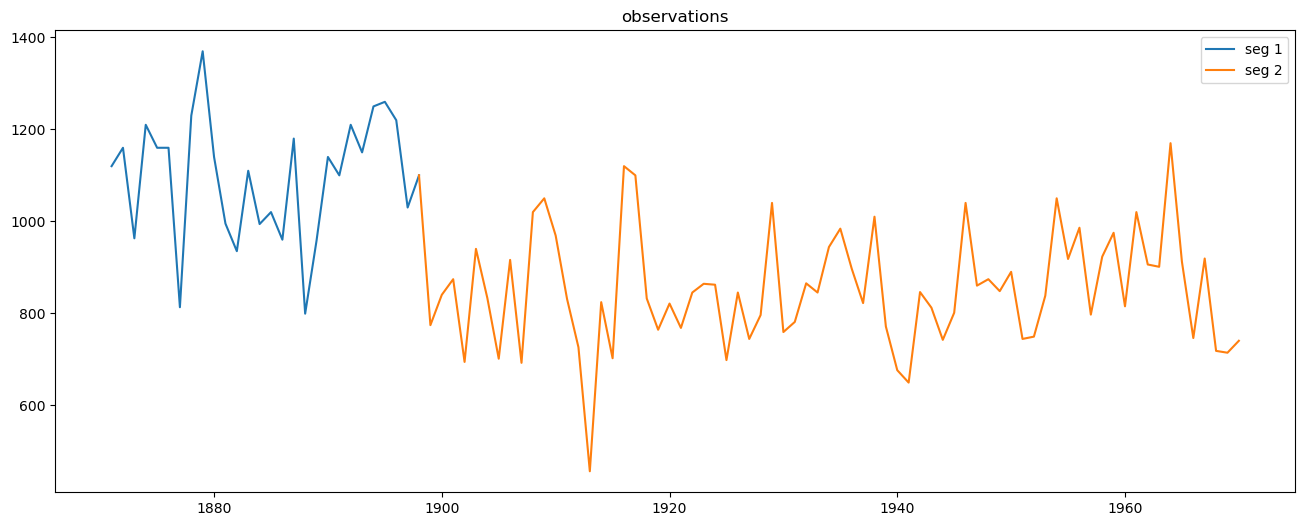
\includegraphics[width=0.9\textwidth]{imgs/nile.png}
\end{figure}
\end{frame}

\begin{frame}
\frametitle{\texttt{harvest} dataset}
\begin{figure}[H]
  \centering
  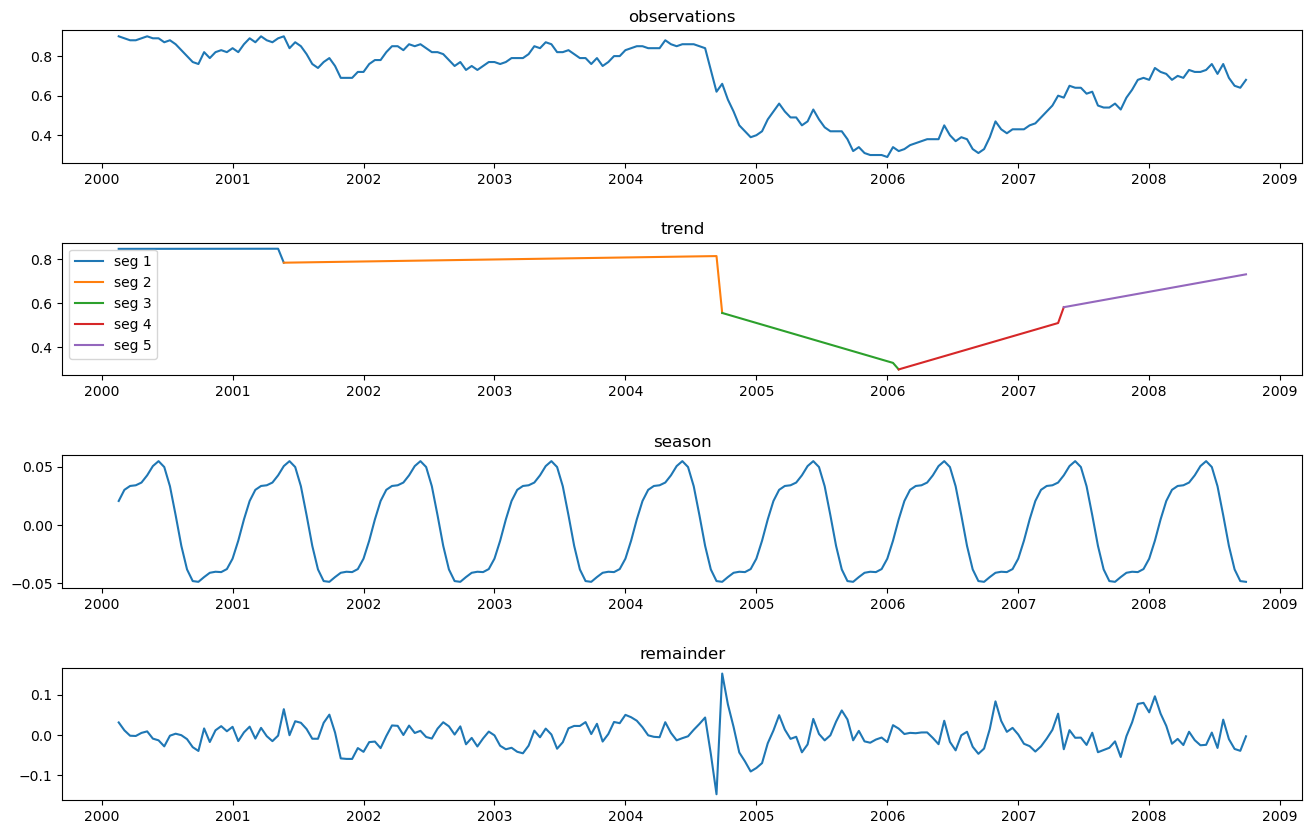
\includegraphics[width=0.9\textwidth]{imgs/harvest.png}
\end{figure}
\end{frame}


\begin{frame}
\frametitle{\texttt{simts} dataset}
\begin{figure}[H]
  \centering
  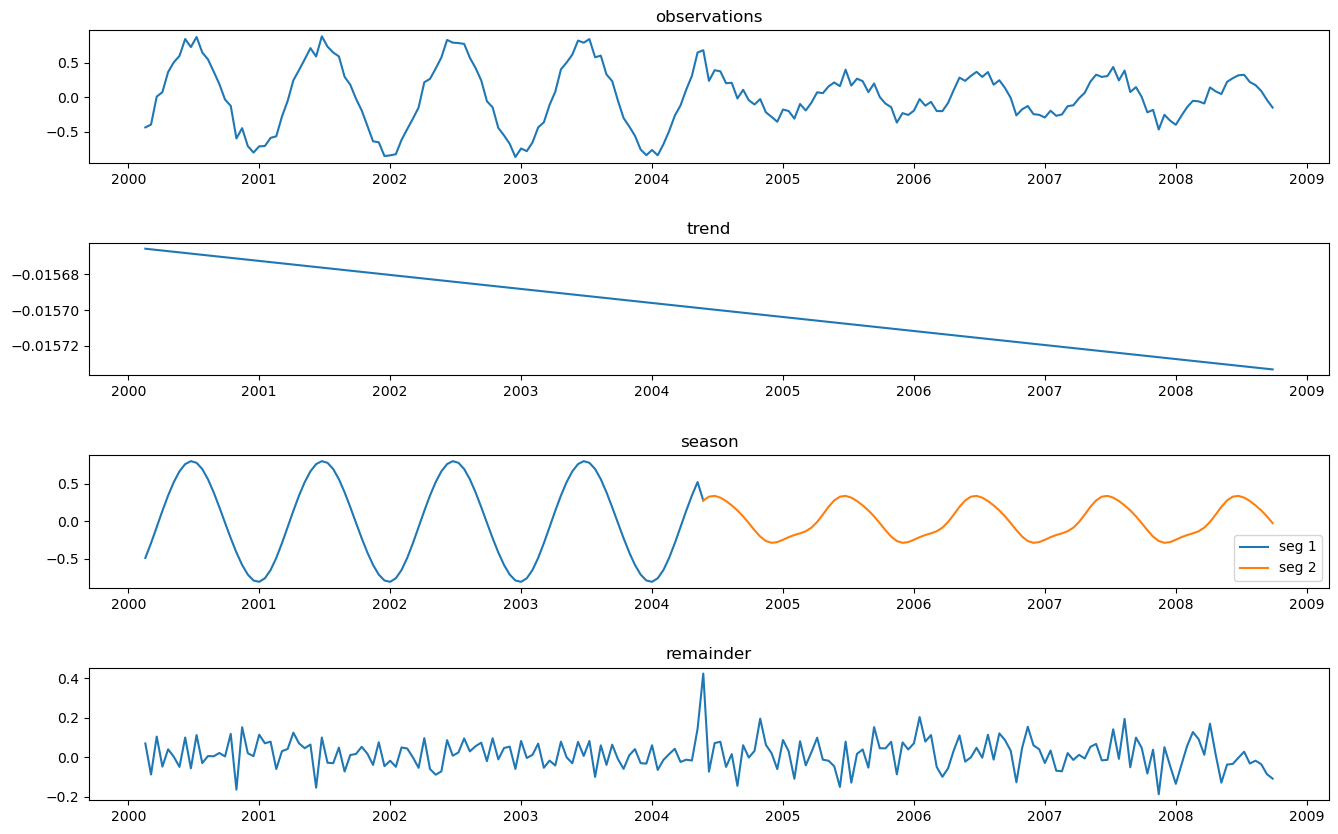
\includegraphics[width=0.9\textwidth]{imgs/simts.png}
\end{figure}
\end{frame}

\begin{frame}
\frametitle{\texttt{ndvi} dataset}
\begin{figure}[H]
  \centering
  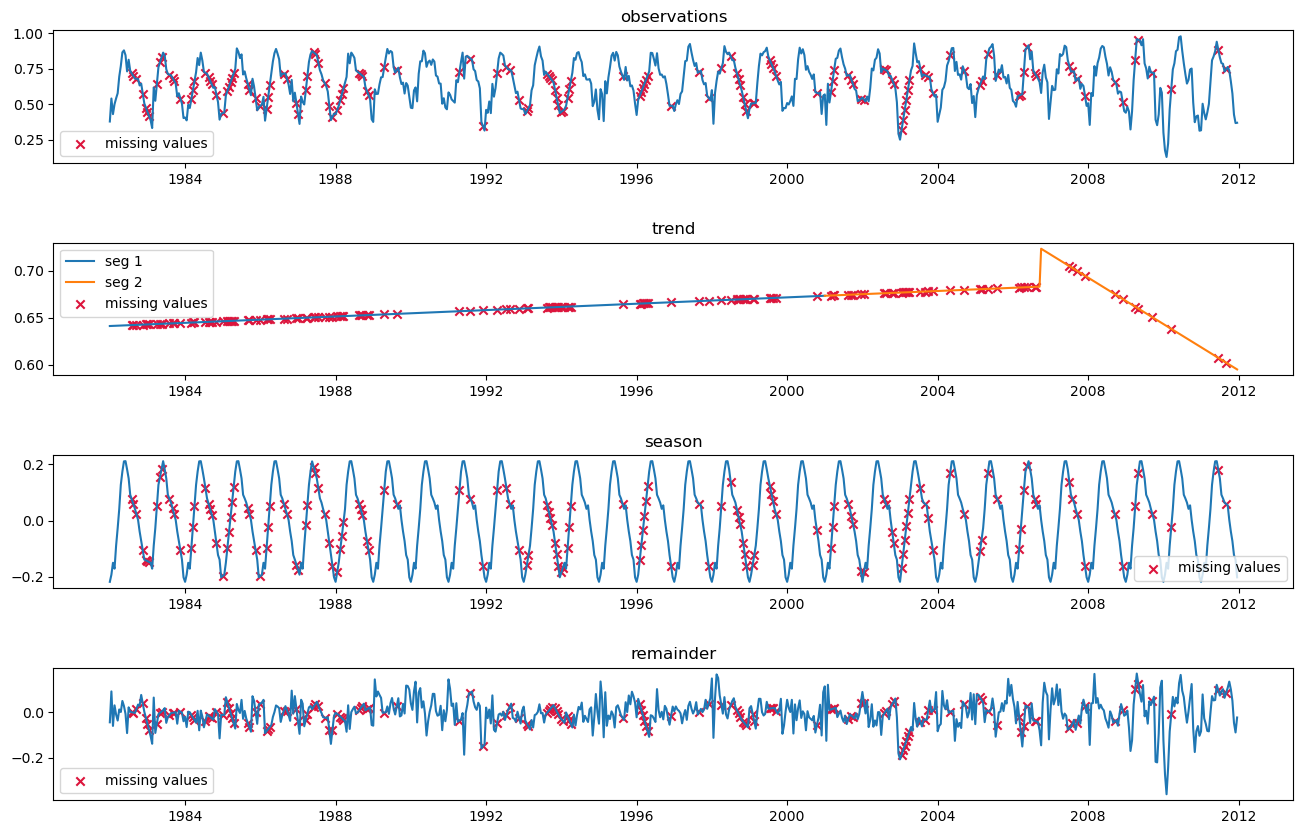
\includegraphics[width=0.9\textwidth]{imgs/ndvi.png}
\end{figure}
\end{frame}

\begin{frame}
\frametitle{Links}
\centering
\begin{itemize}
\item Full project report can be found here:\\
  \url{https://raw.githubusercontent.com/mortvest/bfast-py/master/report/main.pdf}
\item The source code can be found in the GitHub repository:\\
  \url{http://github.com/mortvest/bfast-py}
\end{itemize}
\end{frame}

\begin{frame}
  \frametitle{Questions}
  \centering 
  \Huge ?
\end{frame}

%% \begin{frame}
%%   \frametitle{All results RTX 2080Ti (EXTRA)}
%% \begin{figure}[H]
%%   \centering
%%   \begin{subfigure}[t]{0.4\textwidth}
%%     \centering
%%     \includegraphics[width=\textwidth]{imgs/RTX_2080_Ti_scansubblock.eps}
%%   \end{subfigure}
%%   \begin{subfigure}[t]{0.4\textwidth}
%%     \centering
%%     \includegraphics[width=\textwidth]{imgs/RTX_2080_Ti_flagAggrVal.eps}
%%   \end{subfigure}
%%   \begin{subfigure}[t]{0.4\textwidth}
%%     \centering
%%     \includegraphics[width=\textwidth]{imgs/RTX_2080_Ti_scansubblockexcl.eps}
%%   \end{subfigure}
%% \end{figure}
%% \end{frame}

\end{document}



